\documentclass{article}
\usepackage{graphicx}
\usepackage[margin=1.5cm]{geometry}
\usepackage{amsmath}
\usepackage{hyperref}
\hypersetup{
    colorlinks=true,
    linkcolor=blue,
    filecolor=magenta,      
    urlcolor=cyan,
    pdftitle={Overleaf Example},
    pdfpagemode=FullScreen,
}

\begin{document}
\twocolumn

\title{Tuesday Warm Up, Unit 2: Applications}
\author{Prof. Jordan C. Hanson}
\maketitle

\section{Memory Bank}

\begin{enumerate}
\item \textbf{Cross-correlation}.  Cross-correlation is a measure of similarity of two series as a function of the displacement of one relative to the other.  For discrete, finite signals \( x[n] \) and \( y[n] \), each defined for \( n = 0, 1, \ldots, N-1 \), is given by:
\[
r_{xy}[k] = \sum_{n=0}^{N-1} \bar{x}[n] \cdot y[n+k]
\]
for those values of \( k \) where the summation is well-defined (i.e., \( n+k \) lies within the valid range of \( y[n] \)).  The bar above the signal $x[n]$ represents the complex conjugate.  If $x$ and $y$ are real, $\bar{x} = x$ and $\bar{y} = y$.
\item \textbf{Cross-correlation and the FFT}.  Let $\mathcal{F}(x[n])$ represent the DFT of $x[n]$.  The DFT of the cross-correlation of $x[n]$ and $y[n]$ is
\begin{equation}
\mathcal{F}(r_{xy}[k]) = \overline{\mathcal{F}(x[n])}\cdot \mathcal{F}(y[n]) \label{eq:1}
\end{equation}
That is, the complex conjugate of the DFT of $x[n]$ times the DFT of $y[n]$ is the DFT of the cross-correlation.
\item Like FFT convolution, we can use the above theorem to accelerate cross-correlation calculations.  After computing the right hand side of Eq. \ref{eq:1}, take the real part of the \verb+ifft()+ to find $r_{xy}[n]$.
\end{enumerate}

\section{Cross-Correlation and the FFT}

\begin{enumerate}
\item Using the \verb+xcorr+ function from the \verb+octave+ package \verb+signal+, (a) write code that calculates the \\ cross-correlation between a sine and cosine wave. (b) Show that when the signals are \textit{in phase}, the cross-correlation is maximized. (c) Show that when the signals are \textit{out of phase}, the cross-correlation is mimimized. (d) What phase leads to no correlation? \textit{Hint, consult Fig. \ref{fig:1}.}
\item For the same reason that the basic convolution is computationally slow, cross-correlation is also computationally slow.  In this exercise, FFT cross-correlation will be compared to \verb+xcorr+.  Use the following code to create and normalize two gaussian pulses:
\small
\begin{verbatim}
clear;
close;
home;
pkg load signal

%Define a gaussian pulse
fs = 100.0e6; %Hz
dt = 1/fs; %seconds
T = 100e-6; %seconds
t = dt:dt:T; %seconds
mu1 = 10e-6; %seconds
s1 = 1.0e-6; %seconds
f_c = 1.0e6; %Hz
mu2 = 40e-6; %seconds
s2 = s1;
signal_1 = cos(2*pi*f_c*t).*exp(-0.5*(t-mu1).^2./s1^2);
signal_2 = cos(2*pi*f_c*t).*exp(-0.5*(t-mu2).^2./s2^2);
signal_1 = signal_1/sqrt(sum(signal_1.*signal_1));
signal_2 = signal_2/sqrt(sum(signal_2.*signal_2));
\end{verbatim}
\normalsize
\item Using \verb+[R,lag] = xcorr(signal_2,signal_1)+, find the maxmimum correlation coefficient and the corresponding lag between \verb+signal_1+ and \verb+signal_2+.
\item Repeat the procedure using FFT cross-correlation.  Remember to take the \textit{real} part of the \verb+ifft+ of the product of the \verb+fft()+ of the signal before analyzing it. \textit{Hint:}
\small
\begin{verbatim}
R_fft = real(ifft(conj(fft(signal_1)).*fft(signal_2)));
\end{verbatim}
\item Show that both the standard and FFT cross-correlation produce consistent results.
\end{enumerate}

\begin{figure}
\centering
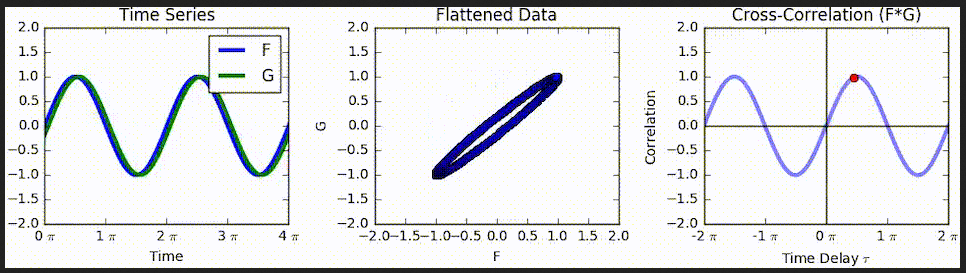
\includegraphics[width=0.4\textwidth]{corr1.png}
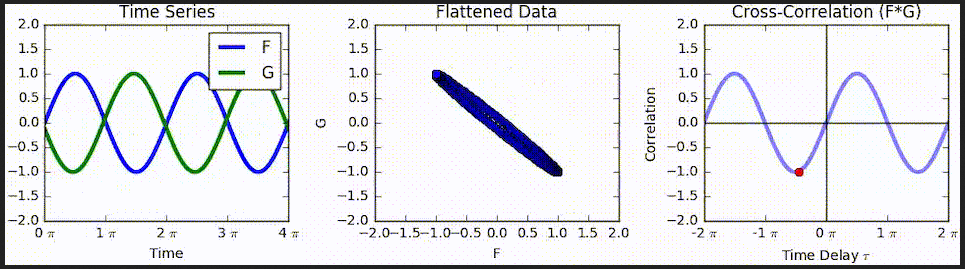
\includegraphics[width=0.4\textwidth]{corr2.png}
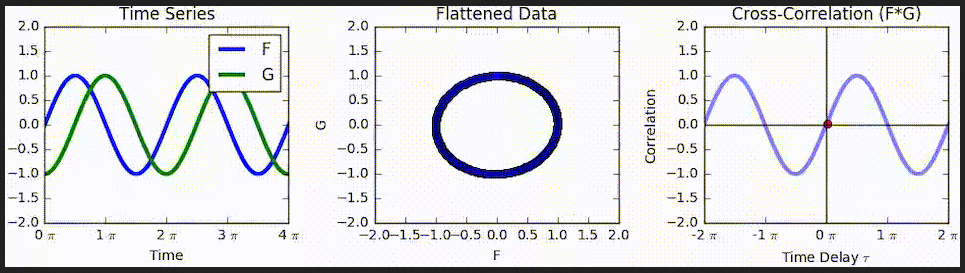
\includegraphics[width=0.4\textwidth]{corr3.png}
\caption{\label{fig:1} (Top) Nearly ideally correlated signals. (Middle) Nearly ideally anti-correlated signals. (Bottom) Uncorrelated signals.  Adapted from \textbf{\href{https://en.wikipedia.org/wiki/Cross-correlation}{Wikipedia: Cross-correlation}}.}
\end{figure}

\end{document}
